\chapter{حل معادلات}
در این فصل ابتدا به نحوه تعریف مثلث بندی می پردازیم. سپس شرایط مرزی را مورد بررسی قرار می دهیم و به این ترتیب آماده ایم تا فضای عناصر متناهی را تعریف کنیم. و در انتها در بخش دوم مسئله را تعریف کرده و به حل آن خواهیم پرداخت.

\section{فضای قابل قبول}
\subsection{ساخت ناحیه $\Omega$}
نواحی در FreeFem++ توسط مرزهای خود تعریف می شوند. به این صورت که ناحیه در سمت چپ مرز قرار دارد. به طور مثال فرض کنیم $\Omega$ ناحیه ای با مرز $ \partial\Omega = [-5,5]\times[-1,1] $ باشد که رأس های آن  A = (-5,-1)، B = (5,-1)، C = (5,1)، D = (-5,1) هستند. حال در گام اول مرزهای AB، BC، CD و DA از $ \partial\Omega $ را با کلمه کلیدی  border مشخص می کنیم. پس از آن می توانیم با کلید واژه buildmesh مثلث بندی $T_{h}$ از $\partial\Omega$ را به طور خودکار تولید کنیم.
\begin{LTR}
	\begin{lstlisting}
 real Dx =.2; // discretization space parameter
 int aa = -5 , bb =5 , cc = -1 , dd =1;
 border AB ( t = aa , bb ) {x = t ;y = cc ; label = 1;};
 border BC ( t = cc , dd ) {x = bb ;y = t ; label = 2;};
 border CD ( t = bb , aa ) {x = t ;y = dd ; label = 3;};
 border DA ( t = dd , cc ) {x = aa ;y = t ; label = 4;};
 mesh Th = buildmesh ( AB ( floor (abs( bb - aa ) / Dx ) ) + BC ( floor ( abs ( dd -  cc ) / Dx ) ) + CD ( floor ( abs ( bb - aa ) / Dx ) ) + DA ( floor (abs( dd - cc ) / Dx )) ) ;
 plot ( AB ( floor ( abs ( bb - aa ) / Dx ) ) + BC ( floor ( abs ( dd - cc ) / Dx ) ) + CD ( floor ( abs ( bb - aa ) / Dx ) ) + DA ( floor (abs( dd - cc ) / Dx )) ) ; // to see the border
 plot ( Th , ps=" mesh.eps ") ; // to see and save the mesh
	\end{lstlisting}
\end{LTR} 
نتیجه اجرای کد بالا به صورت زیر است :

\begin{figure}[hbt!]
	\centering
	\begin{subfigure}{.5\textwidth}
		\centering
		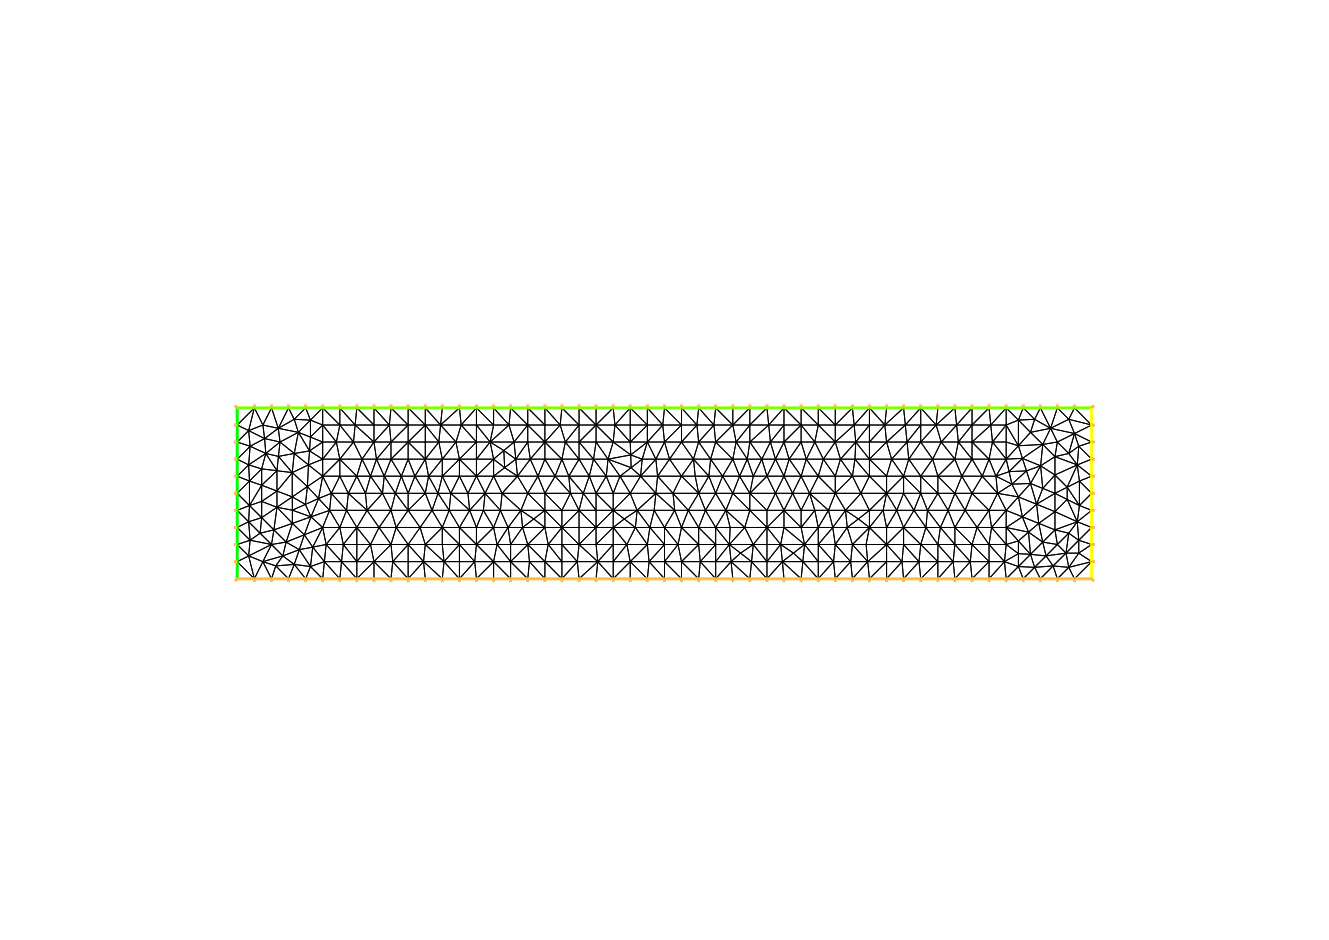
\includegraphics[width=.5\linewidth]{1}
		\caption{مرز ناحیه $\Omega$}
		%\label{fig:مرز ناحیه $\Omega$}
	\end{subfigure}%
	\begin{subfigure}{.5\textwidth}
		\centering
		
\includegraphics[width=.5\linewidth]{2}
		\caption{مثلث بندی ناحیه $\Omega$}
		%\label{fig مثلث بندی ناحیه $\Omega$}
	\end{subfigure}
	\caption{رسم ناحیه $\Omega$ و مثلث بندی آن}
	%\label{fig:رسم ناحیه $\Omega$ و مثلث بندی آن}
\end{figure}
 راه دیگر برای ساخت یک دامنه مربعی با مثلث بندی یکسان به صورت زیر است :
\begin{LTR}
	\begin{lstlisting}
 int m=3;
 int n=6;
 mesh Th = square (m ,n ,[x,y]) ; // build a square with m point on x direction and n point on y direction
 mesh Th1 = movemesh ( Th ,[x*2 ,y+1]) ; // translate the square [0 ,1]*[0 ,1] to a rectangle [0 ,2]*[1 ,2]
 savemesh ( Th1 ,"mesh.msh") ; // to save the mesh
 mesh Th2 ("mesh.msh") ; // to load the mesh
 plot(Th2);
	\end{lstlisting}
\end{LTR} 
نتیجه کد بالا به صورت زیر خواهد بود :
\begin{figure}[hbt!]
	\centering
	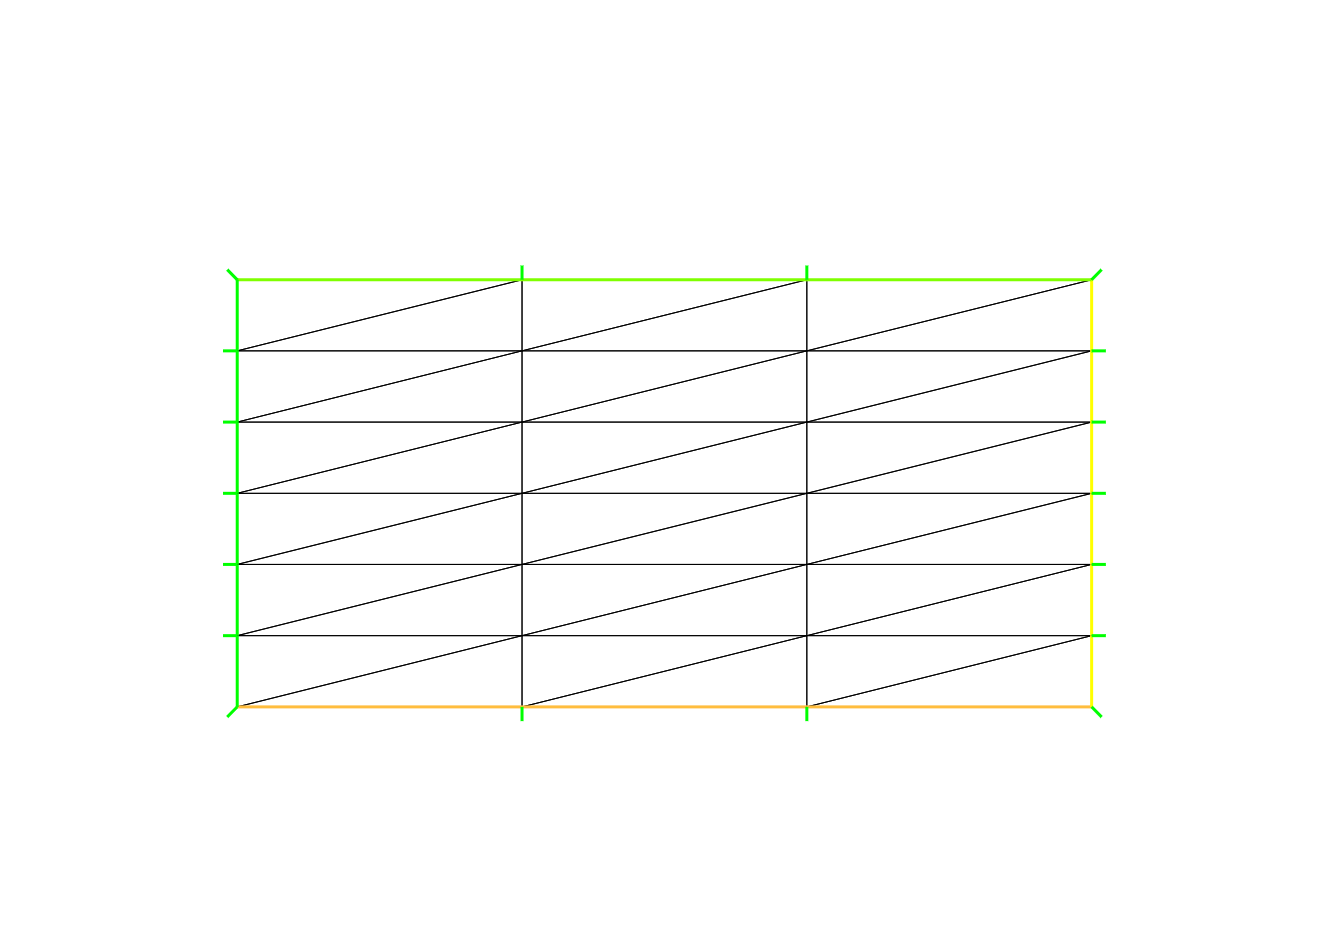
\includegraphics[width=\linewidth]{3}
	\caption{ ناحیه $\Omega$}
\end{figure}
همچنین ما می توانیم ناحیه خود را به صورت پارامتری تعریف کنیم :
\begin{LTR}
	\begin{lstlisting}
 border C(t = 0, 2*pi ){ x = cos(t); y = sin(t); label=1; }
 mesh Th = buildmesh(C(50)) ;
 plot(Th);
	\end{lstlisting}
\end{LTR} 
که نتیجه اش به صورت زیر خواهد بود :

\begin{figure}[hbt!]
	\centering
	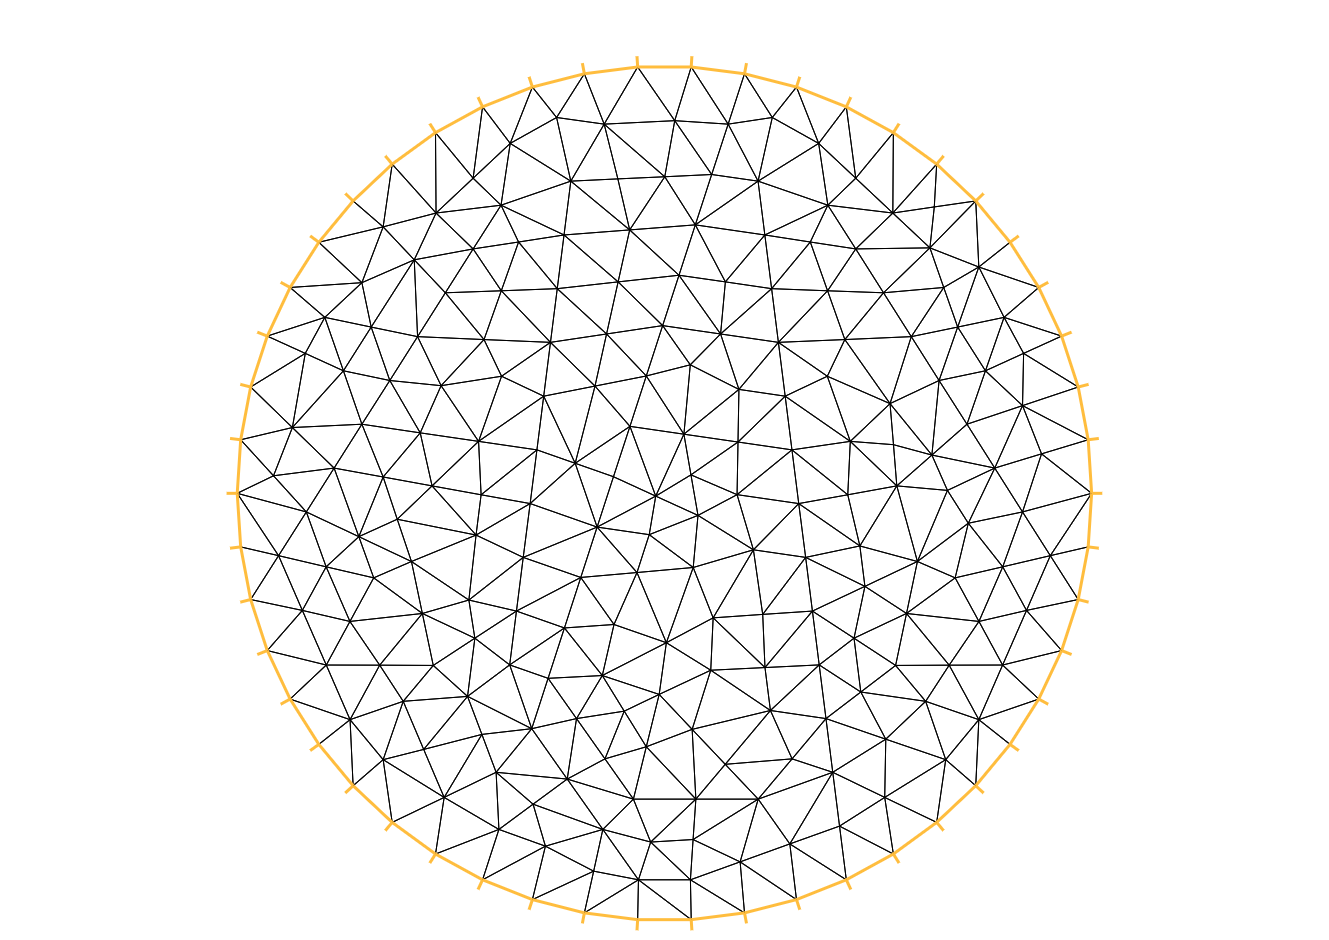
\includegraphics[width=\linewidth]{4}
	\caption{ تعریف ناحیه $\Omega$ به صورت پارامتری}
\end{figure}

\subsection{فضای عناصر متناهی}
عموما یک فضای عناصر متناهی عبارت است از فضای چندجمله ای های روی $T_{h}$ که دارای یک سری خواص معین باشند. ما یک فضای عناصر متناهی را به صورت 
\begin{LTR}
	\begin{lstlisting}
 fespace Vh ( Th , P1 ) ;
	\end{lstlisting}
\end{LTR}
تعریف می کنیم. تاکنون انواع فضاهای عناصر متناهی قابل دسترس عبارت اند از :
\begin{enumerate}
	\item P0
	\item  P03d
	\item  P1
	\item  P13d
	\item  P1dc
	\item  P1b
	\item  P1b3d
	\item  P2
	\item  P23d
	\item  P2b
	\item  P2dc
	\item  P3
	\item  P3dc
	\item  P4
	\item  P4dc
	\item  Morley
	\item  P2BR
	\item  RT0
	\item  RT03d
	\item  RT0Ortho
	\item  Edge03d
	\item  P1nc
	\item  RT1
	\item  RT1Ortho
	\item  BDM1
	\item  BDM1Ortho
	\item  TDNNS1
\end{enumerate}
که برای مثال P0 به صورت\\
$P0_{h} := \{ v \in L^{2}(\Omega) | \forall K \in T_{h} \exists \alpha_{K} \in \mathbb{R} : v|_{K} = \alpha_{K} \}$\\
تعریف می شود.
\subsection{شرایط مرزی}
برای تعریف شرط مرزی دیریکله روی مرز $ \Gamma_{d}  \subsetneq \mathbb{R} $ به صورت $u_{\Gamma_{d}} = f_{d}$ می توانیم به صورت on(gammad , u=f) عمل کنیم که u تابع مجهول است.
\section{حل مسئله}
ما روش های مختلف حل را برای معادله پواسون بررسی خواهیم کرد. این معادله به صورت زیر تعریف می شود: 
تابع $ u := \Omega \rightarrow \mathbb{R} $ را چنان بیابید که برای تابع $f\in L^{2}(\Omega)$ داده شده را چنان بیابید که در\\



\[   
\begin{cases}
-\bigtriangleup u=f &\quad\text{in } \Omega\\
u = 0 &\quad\text{on } \partial \Omega\\ 
\end{cases}
\]\\
صدق کند. فرم تغییراتی این مسئله به صورت یافتن $u \in H^{1}_{0}(\Omega)$ به قسمی که به ازای هر $v \in H^{1}_{0}(\Omega)$ تساوی\\ 
\[   
a(u,v) = l(v) 
\]\\
که در آن
\[
\begin{cases}   
a(u,v) = \int_{\Omega} \bigtriangledown u \cdot \bigtriangledown v dxdy\\
l(v) = \int_{\Omega} f \cdot v dxdy
\end{cases}
\]\\
است نوشته می شود.\\
حال فرض کنیم $T_{h}$ یک مثلث بندی هموار از $\Omega$ با مثلث های از اندازه حداکثر $h<1$ باشد. همچنین فرض کنیم \\
\[
V_{h} := \{ v_{h} \in C^{0}(\bar{\Omega}); v_{h}|_{T} \in \mathbb{P}_{1}(T) , \forall T \in T_{h}; v_{h} = 0 \text{on }\partial\Omega \}
\]\\
یک زیر فضای عناصر متناهی از $ H^{1}_{0}(\Omega)$ است و $\mathbb{P}_{1}$ مجموعه چندجمله ای های درجه کمتر یا مساوی یک روی $\mathbb{R}$ است و بنابراین فرم ضعیف معادله پواسون عبارت است از پیدا کردن $u_{h} \in V_{h}$ به قسمی که به ازای هر $v_{h} \in V_{h}$ در معادله\\
\[   
\int_{\Omega} \bigtriangledown u_{h} \cdot \bigtriangledown v_{h} dxdy - \int_{\Omega} f \cdot v_{h} dxdy = 0
\]\\
صدق کند.
\subsection{دستور solve}
اولین شیوه حل معادله، تعریف و حل به صورت هم زمان به صورت زیر است.
\begin{LTR}
	\begin{lstlisting}
 solve poisson ( uh , vh , init =i, solver = LU ) = // Solve Poisson Equation
	int2d ( Th ) ( Grad ( uh ) ’* Grad ( vh ) ) // bilinear form
	-int2d ( Th ) ( f * vh ) // linear form
	+on (1 ,2 ,3 ,4 , uh =0) ; // Dirichlet B.C.
	\end{lstlisting}
\end{LTR}
\subsection{دستور problem}
در این روش ابتدا مسئله را با دستور problem تعریف و سپس با فراخوانی نام تخصیص داده شده به حل آن اقدام می کنیم.
\begin{LTR}
	\begin{lstlisting}
 problem poisson (uh , vh , init =i, solver = LU ) =// Definition of the problem
	int2d ( Th ) ( Grad ( uh ) ’* Grad ( vh ) ) // bilinear form
	-int2d ( Th ) ( f * vh ) // linear form
	+on (1 ,2 ,3 ,4 , uh =0) ; // Dirichlet B.C.
 Poisson ; // Solve Poisson Equation
	\end{lstlisting}
\end{LTR}

